\documentclass[a4paper,10pt]{article}

\usepackage{datetime}
\usepackage{fullpage}
\usepackage{indentfirst}
\usepackage{amsmath}
\usepackage{amsfonts}
\usepackage{amssymb}
\usepackage{bm}
\usepackage{enumerate}
\usepackage{listings}
\usepackage{graphicx}
\usepackage{float}

\linespread{1.5}

\begin{document}
\title{Answers to the theory questions - Homework 2 \\
  \large Computer Vision (2016 Spring)}
\author{2009-11744 Gyumin Sim}
\maketitle

\section*{Question 1}

Assume the intensity of each light source is $I$,
the normal of a point on the surface is $\vec{n}$,
and the albedo of the surface is $\rho$.
Then, the surface radiance of the point will be
\begin{align*}
L &= \frac{\rho}{\pi} I \vec{n} \cdot \vec{s_1} + \frac{\rho}{\pi} I \vec{n} \cdot \vec{s_2} \\
&= \frac{\rho}{\pi} I \vec{n} \cdot ( \vec{s_1} + \vec{s_2} ) \\
&= \frac{\rho}{\pi} I || \vec{s_1} + \vec{s_2} || \vec{n} \cdot \frac{ \vec{s_1} + \vec{s_2} }{ || \vec{s_1} + \vec{s_2} || }.
\end{align*}
The illumination will be same as if there is an effective light source $s_3$, the direction of which is
$( \vec{s_1} + \vec{s_2} ) / || \vec{s_1} + \vec{s_2} || $,
and the intensity of which is
$I || \vec{s_1} + \vec{s_2} ||$.

If the light sources $s_1$ and $s_2$ have unequal intensities $I_1$ and $I_2$,
the surface radiance of a point will be
\begin{align*}
L &= \frac{\rho}{\pi} I_1 \vec{n} \cdot \vec{s_1} + \frac{\rho}{\pi} I_2 \vec{n} \cdot \vec{s_2} \\
&= \frac{\rho}{\pi} \vec{n} \cdot ( I_1 \vec{s_1} + I_2 \vec{s_2} ) \\
&= \frac{\rho}{\pi} || I_1 \vec{s_1} + I_2 \vec{s_2} || \vec{n} \cdot \frac{ I_1 \vec{s_1} + I_2 \vec{s_2} }{ || I_1 \vec{s_1} + I_2 \vec{s_2} || }.
\end{align*}
So, the direction of the effective source will be
$( I_1 \vec{s_1} + I_2 \vec{s_2} ) / || I_1 \vec{s_1} + I_2 \vec{s_2} ||$,
and its intensity will be
$|| I_1 \vec{s_1} + I_2 \vec{s_2} ||$.

\section*{Question 2}

\begin{figure}[H]
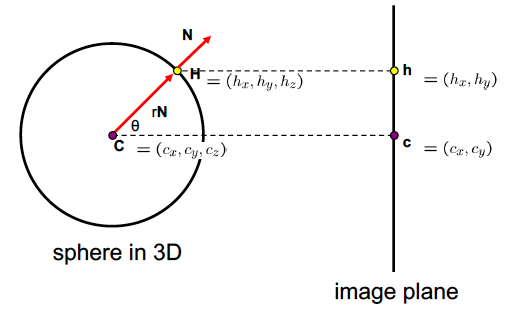
\includegraphics[width=0.6\textwidth]{sphere}
\centering
\caption{A sphere in 3D and the image plane (the figure from page 29 of lec08)}
\label{fig:sphere}
\end{figure}

Let $xy$-axis be along with the image axis, and assume the image plane is on a negative $z$-coordinate.
See figure~\ref{fig:sphere}.
Let $(c_x, c_y, c_z) = (0, 0, 0)$, and $r = R$.
Then, $(h_x, h_y)$ happens to be $(u - a, v - b)$.
From the equation $||\bm{H} - \bm{C}|| = r$, get $h_z$ as follows
\begin{align*}
&& \sqrt{ (u-a)^2 + (v-b)^2 + h_z^2 } &= R \\
&\Rightarrow& (u-a)^2 + (v-b)^2 + h_z^2 &= R^2 \\
&\Rightarrow& h_z &= - \sqrt{ R^2 - (u-a)^2 - (v-b)^2 }.
\end{align*}
Finally, get $\bm{N}$ from the equation $\bm{H} - \bm{C} = r \bm{N}$,
\begin{align*}
&& (u-a, v-b, - \sqrt{ R^2 - (u-a)^2 - (v-b)^2 }) &= R \bm{N} \\
&\Rightarrow& \frac{1}{R} (u-a, v-b, - \sqrt{ R^2 - (u-a)^2 - (v-b)^2 }) &= \bm{N}.
\end{align*}

\end{document}
